\chapter{Crystallography and Point Defects}

\label{ch:crystallography}

\section{\zirconia\ phases and stabilisation}

\zirconia\ is unusual in exhibiting three commonly reported polytypes in its binary phase diagram (Figure \ref{figure:binary_phase_diagram}). Each will now be described and contrasted.

\begin{figure}[htp]
\centering
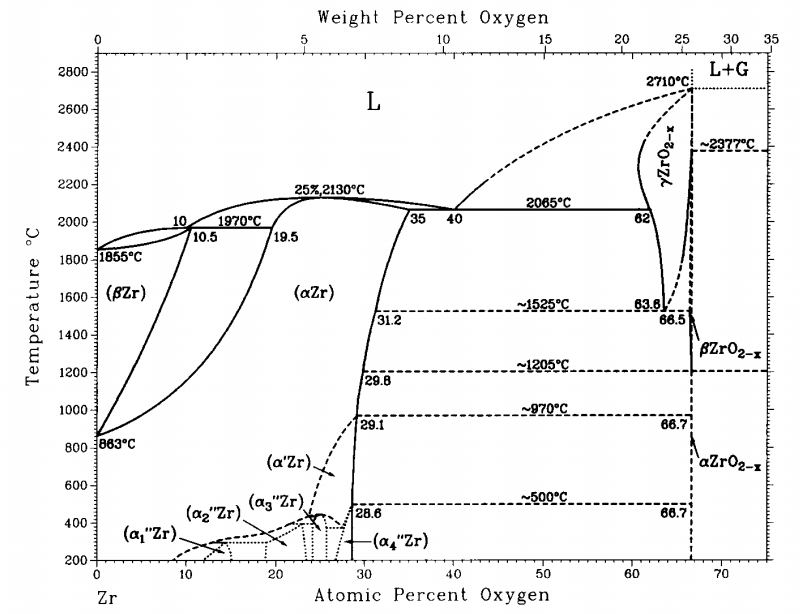
\includegraphics[height=9cm]{images/zro2_binary_phase.png}
\caption{Binary phase diagram of the Zr and O$_{2}$ system. Taken from \cite{Abriata1986TheSystem}.}
\label{figure:binary_phase_diagram}
\end{figure}

\subsection{Monoclinic}

A unit cell of monoclinic \zirconia\ is illustrated in Figure \ref{figure:coordination}. The dashed line (approximately 3.7\r{A} in length) shows the Zr-O bond which is broken when transitioning to monoclinic from the tetragonal phase.

\begin{figure}[htp] % Mono coordination figure
\centering
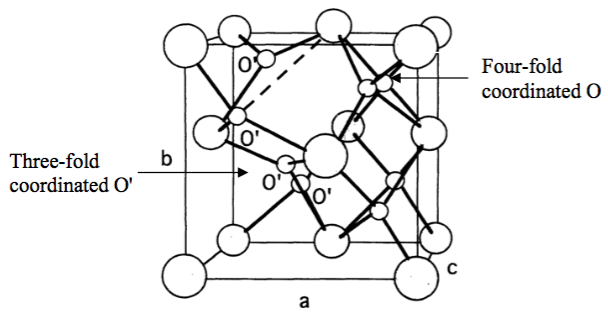
\includegraphics[height=6.2cm]{images/coordination.png}
\caption{A monoclinic zirconia unit cell indicating the two different oxygen bond coordinations. Small spheres represent oxygen ions while large spheres represent zirconium ions. Taken from \cite{Xia2010}.
\label{figure:coordination}}
\end{figure}

\begin{figure}[htp] % Mono Zr centre
\centering
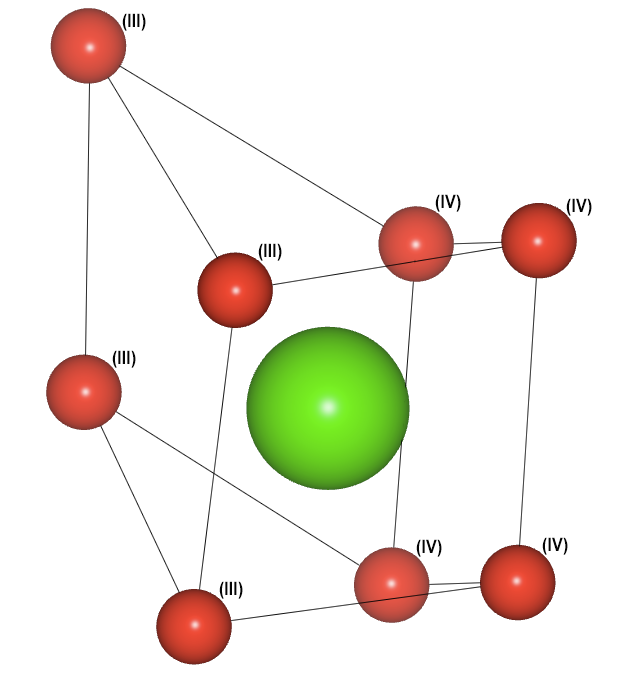
\includegraphics[height=6cm]{images/zr_centre_mono.png}
\caption{Zirconium centre in monoclinic \zirconia\ showing nearest oxygen atoms and their respective bond co-ordinations. Zirconium atoms are shown in green and oxygen atoms in red.}
\label{figure:monoschottky}
\end{figure}


\begin{table}[htp]
\centering
\onehalfspacing
\caption{\zirconia\ crystal structures and their stable temperatures at 1 atm \cite{Howard1988}.}
\label{table:phases}
\begin{tabular}{ccc}
\hline
{Crystal Structure} & {Space Group}    & {Temperature Range (K)} \\ \hline
\multicolumn{1}{c}{Monoclinic} & \multicolumn{1}{c}{$P2_1/c$} & \multicolumn{1}{c}{$T$ \textless\ 1440}     \\
\multicolumn{1}{c}{Tetragonal} & \multicolumn{1}{c}{$P4_2/nmc$} & \multicolumn{1}{c}{1440 \textless\ $T$ \textless\ 2640}        \\
\multicolumn{1}{c}{Cubic} & \multicolumn{1}{c}{$Fm\overline{3}m$}     & \multicolumn{1}{c}{2640 \textless\ $T$ \textless\ 2950}      \\ \hline
\end{tabular}
\end{table}

\subsection{Tetragonal}

\subsection{Cubic}

\subsection{Other phases}

\subsubsection{Cotunnite}

Two orthorhombic phases of \zirconia\ have also been observed at high pressures.

\begin{figure}[htp]
  \centering
      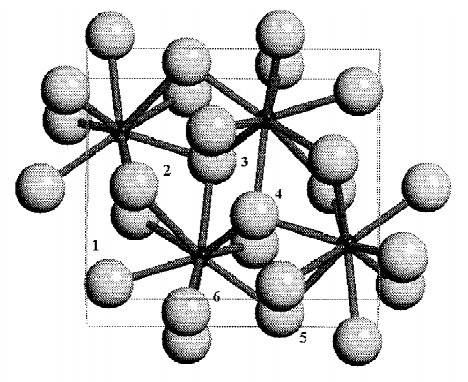
\includegraphics[height=9cm]{images/cotunnite_structure.png}
  \caption{Illustration of the OII cotunnite crystal structure of \zirconia . Zirconium and oxygen ions are shaded dark and light respectively. Taken from \cite{Haines1997CharacterizationHafnia}.}
  \label{fig:cotunnite_structure}
\end{figure}

\subsubsection*{Volume expansion}

The phase transitions in \zirconia\ are accompanied by a change in volume, where the monoclinic phase is the least dense and the cubic phase is the most dense (see Figure \ref{figure:zrobonddistance}). This is especially significant in the case of the martensitic t-\zirconia\ to m-\zirconia\ transition, where the volume increases by around 9\% \cite{Gupta1977}. This has substantial implications for the creation and opening of cracks as \zirconia\ is a ceramic material with low toughness. This is especially relevant in a reactor scenario where temperature cycling (shutdown/startup or load-following behaviour) may lead to fatigue if the phase transition threshold is passed.

Another consequence of this large volume expansion is that a significant hysteresis effect is observed in the monoclinic/tetragonal phase transition, as shown in Figure \ref{fig:phasediagram}. 
%as the resulting coherency strain is likely to result in reduced mobility of fission products that have been embedded in the bulk crystal. 

\begin{figure}[htp]
  \centering
      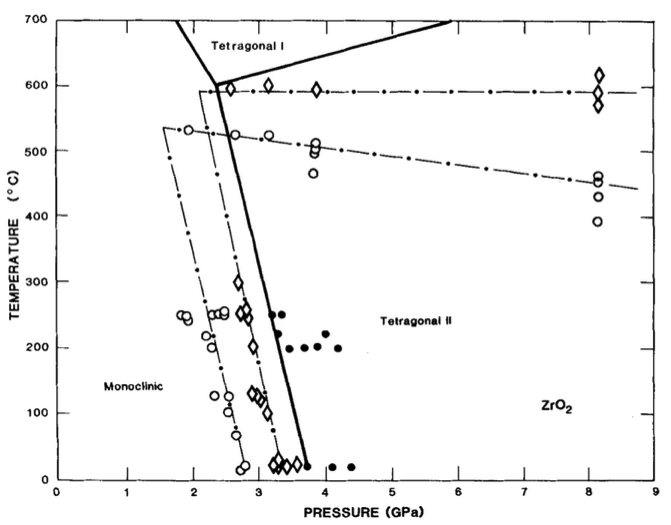
\includegraphics[height=10cm]{images/zirconiaphasediagram.png}
  \caption{Pressure-temperature phase diagram for \zirconia . Dash-dotted lines represent more recent data. Diamonds mark transition points during an increase in pressure/temperature, while open circles are used for a decrease in pressure/temperature. Solid circles represent transition points for a fresh, single crystal sample. Taken from \cite{gando2011partial}. \label{fig:phasediagram}}
\end{figure}

\begin{figure}
\begin{center}
\begin{tikzpicture}
	\begin{axis}
		[width=12cm, xlabel={Nearest neighbour Zr-O bond distance (\r{A})}, ylabel={Relative occurrence}, ymin=0, ymax=140, xmin=2.0, xmax=2.50, legend style={{draw=}, at={(0.95,0.95)}, anchor=north east, legend columns=1}]
		\addplot[no marks] table [x=zr_o_dist, y=monoclinic,]{dat/zr_o_bond_distances.dat}; \addlegendentry{Monoclinic};
        \addplot[no marks, dashed] table [x=zr_o_dist, y=tetragonal, ]{dat/zr_o_bond_distances.dat}; \addlegendentry{Tetragonal};
        \addplot[no marks, densely dotted] table [x=zr_o_dist, y=cubic,]{dat/zr_o_bond_distances.dat}; \addlegendentry{Cubic};
			\end{axis}
		\end{tikzpicture}
		\caption{Density plot of the nearest neighbour Zr-O bond distances in \zirconia\ for each crystal structure. Specific volumes from DFT simulations are 11.99 \r{A}$^{3}$ion$^{-1}$, 11.51 \r{A}$^{3}$ion$^{-1}$, and 11.13 \r{A}$^{3}$ion$^{-1}$ for monoclinic, tetragonal, and cubic phases respectively.}
		\label{figure:zrobonddistance}
	\end{center}
\end{figure}


\subsection{Pressure stabilisation (isochoric + autostabilisation)}

The tetragonal and cubic phases of \zirconia\ are stabilised at high pressure. Since the oxide has a larger volume than the underlying metal (pilling-bedworth ratio of 1.5X), the growth of the oxide will itself impose stresses which may stabilise the tetragonal phase.

\subsection{Dopant stabilisation (lower valence cations)}

Some dopants will also stabilise the tetragonal and cubic phases of \zirconia. The most technologically significant of which is yttrium, which at concentrations of 15\% (atomic), fully stabilises the cubic phase. Zirconia stabilised this way is known as yttria-stabilised zirconia (YSZ). The way this works is by trivalent yttrium promoting the inclusion of charge compensating oxygen vacancy defects (see equation XXX). This works in a similar way with several other cation dopants such as trivalent scandium and divalent magnesium.

\section{Point Defects}

\subsection{Kr\"{o}ger-Vink notation}

Kr\"{o}ger-Vink notation \cite{kroger1956relations} is used throughout this thesis to describe defects. It is widely used in physical chemistry and is a useful shorthand for describing chemical reactions where conservation of mass, charge and lattice sites is required. The notation syntax is of the form \ch{x^{y}_{z}}, where x is the substituted atom or missing atom (i.e. a vacancy V), y is the charge of the defect (relative to the lattice species that originally occupied the site) and z is the site the defect occupies. Positive and negative charges are indicated with dots (\ch{^{*}}) and dashes (\ch{^{'}}) respectively, otherwise a cross (\ch{^{x}}) is used to denote a neutral defect. The site may be either a lattice site (such as Zr or O in \zirconia ) or an interstitial site ($i$). Table \ref{table:krogervink} shows examples of several different types of defects and their respective Kr\"{o}ger-Vink notation.

\begin{table}[htp] % Kroger-Vink notation table
\onehalfspacing
\centering
\caption{Examples of Kr\"{o}ger-Vink notation for several defects in \zirconia .}
\label{table:krogervink}
\begin{tabular}{cc}
\hline
Defect & Kr\"{o}ger-Vink Notation \\ \hline
Anion vacancy & \ch{V_{O}^{**}} \\
Cation vacancy & \ch{V_{Zr}^{''''}} \\
Anion interstitial & \ch{O_{i}^{''}} \\
Cation interstitial & \ch{Zr_{i}^{****}} \\
Iodine (I$^{-}$ anion) on oxygen site & \ch{I_{O}^{*}} \\ \hline
\end{tabular}
\end{table}

